\documentclass[border=3mm]{standalone}

\usepackage{tikz}
\usetikzlibrary{arrows,shapes.gates.logic.US,shapes.gates.logic.IEC,calc}
\begin{document}
\thispagestyle{empty}
\tikzstyle{branch}=[fill,shape=circle,minimum size=15pt,inner sep=0pt]
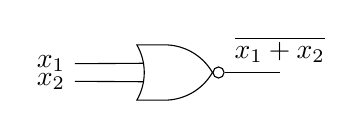
\begin{tikzpicture}[label distance=2mm]

        \node (x1) at (0,0) {$x_1$};
    \node (x2) at (0,-.22) {$x_2$};

    \node[nor gate US, draw, logic gate inputs=nn , minimum size=20pt] at ($(x1)+(1.5,-.11)$)  (And1) {};

    \draw (x1) -- (And1.input 1);
    \draw (x2) -- (And1.input 2);
    \draw (And1.output) -- ([xshift=.7cm]And1.output) node[above] {$\overline{x_1 + x_2}$};
\end{tikzpicture}
\end{document} 
